\section{Stack (Pila)}
Le pile sono delle strutture dati con organizzazione {\textbf{LIFO}}
(Last-In-First-Out).\newline
Possono essere implementate tramite array o tramite liste lineari. Sono
preferibili le liste concatenate singolarmente. \\[2pt]

\begin{wrapfigure}{r}{7cm}
    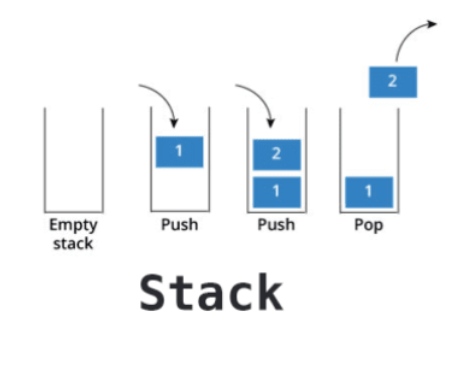
\includegraphics{stack.png}
\end{wrapfigure}


Le operazioni che possono essere eseguite su una pila sono:
\begin{itemize}
    \item {\texttt{isEmpty() $\rightarrow$ boolean}} restituisce \verb|true| se la pila è vuota, \verb|false| altrimenti
    \item {\texttt{push(elemento)}} aggiunge un elemento alla pila
    \item {\texttt{pop() $\rightarrow$ elemento}} rimuove il primo elemento dalla pila e lo restituisce
    \item {\texttt{top() $\rightarrow$ elemento}} restituisce il primo elemento della pila
\end{itemize}


\begin{algorithm}
    \caption{isEmpty}
    \Indm{\textbf{Funzione}} {\emph{isEmpty}}() $\rightarrow$ {\emph{boolean}}\\
       \Indp\eIf{$top = null$}{\Return{$true$}}{\Return{$false$}}
\end{algorithm}

\begin{algorithm}
    \caption{push}
    \Indm\textbf{Procedura} \emph{push}(elemento \emph{x})\\
    \Indp$r$ $\leftarrow$ riferimento ad un nuovo nodo\\
    $r.dato$ $\leftarrow$ $x$\\
    $r.pros$ $\leftarrow$ $top$\\
    $top$ $\leftarrow$ $r$\\
    
\end{algorithm}

\begin{algorithm}
    \caption{top}
    \Indm\textbf{Funzione} \emph{top}() $\rightarrow$ elemento\\
    \Indp\Return{$top.dato$}
\end{algorithm}
\text{}\\[30pt]

\begin{algorithm}
    \caption{pop}
    \Indm\textbf{Funzione} \emph{pop}() $\rightarrow$ elemento\\
    \Indp$x$ $\leftarrow$ $top.dato$\\
    $top$ $\leftarrow$ $top.pros$\\
    \Return{$x$}
\end{algorithm}